\textit{Introduce topic by talking about cells. Attention grabber, relate biophysics study to cancer reserach and many areas where we need to focus our research. Short and sweet, maybe 1 or 2 short paragraphs.}

	Neuroegenerative diseases, such as Alzheimer's and Huntinton's disease, have consistently been one of the leading causes of death in the United States. Scientists all over the world struggle to find the leading causes of these diseases and continue to hope for a breakthrough in science in attempt to prevent or even cure these fatal diseases. Although this breakthrough has yet to come, researchers discovered that one of the central causes of cell degeneration is motor protein failure. More specifically, defects in the motor protein dynein has been linked to neurodegeneration due to the cell's funtional dependence on dynein and its mechanical properties. However, unlike dynein's motor protein siblings, dynein possesses a unique structure causing it to stochasitcally move around the cell and unpredicatable in nature. Thus, fully understandding the mechanisms of dynein can allow us to further conclude causes of its failure, putting us one step closer to solving the breakthrough. 

\section{Background}

\begin{figure}[H]
	\centering
	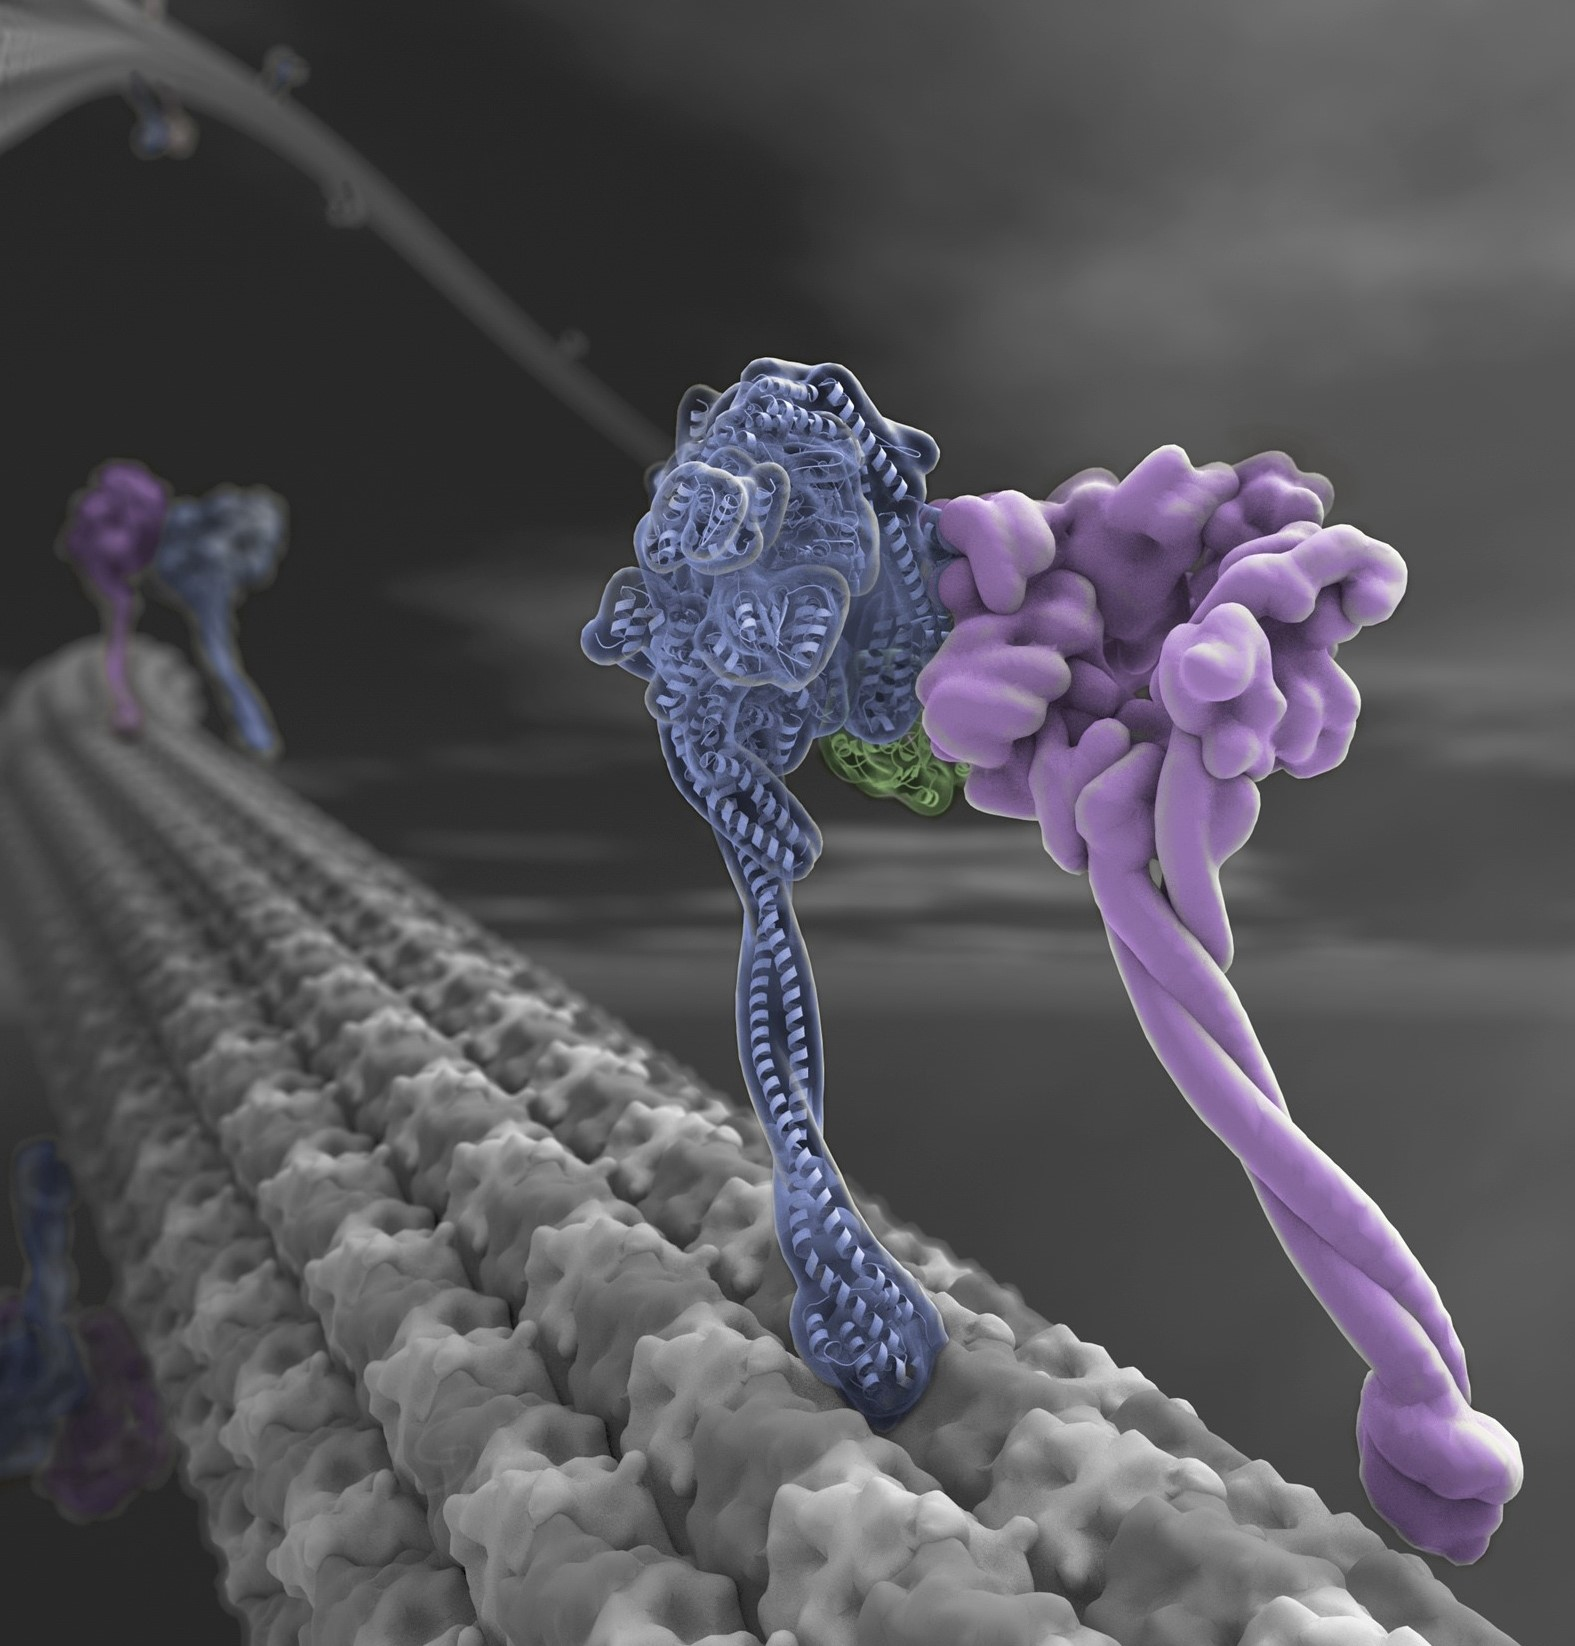
\includegraphics[width=0.6\columnwidth]{Figures/dynein_walking_art.jpg}
	\caption[Artist Rendition of Dynein]{\textbf{Artist Rendition of Dynein} \cite{JohnsonArt}}
	\label{fig:final_disp}
\end{figure}

Cells are complicated. Despite their degeneracies, cells have the ability to move, perfectly divide, and spatially organize themselves. They are constructed by organelles surrdounded by a network of protein filaments called the cytoskeleton. The cytoskeleton is composed of microtubules (MT) that act as a walkway for motor protein soldiers to carry out the functions of the cell. These motor proteins consists of kinesin, myosin, and dynein. 


\textit{THIS IS STRAIGHT FROM PROPOSAL, NEED TO FIX THIS AND ADJUST SO THAT MORE DYNEIN DETAILS GOES INTO CHAPTER 2}

In a eukaryotic cell, dynein is one of the three motor proteins that are responsible for the cell’s ability to move, divide, and spatially organize itself. Similar to the more researched kinesin, dynein conveys cargo along the microtubule track by using ATP to power its two binding domains (its “feet”). However, its walking-like movements along the track are very unpredictable and can vary in terms of distance and direction. Dynein’s two feet can also act independently from each other causing much more erratic and stochastic steps. However, despite dynein’s stochastic nature, dynein is still able to achieve processive motion due to the functions of its structure. Structurally, dynein is composed of two motor heavy chain subunits of linked amino acids, called polypeptides, each which are separated into domains. These domains are the tail domain, the linker domain, the six AAA+ domains, and the microtubule binding domains (See Figure 1). The AAA+ domains are responsible for ATP hydrolysis, in which converts chemical energy stored in ATP into mechanical work causing dynein’s motility. 

Because dynein’s stepping is unpredictable in nature, its stepping mechanism has not been intensely studied as compared to its structure. Questions regarding the electrostatic interactions with the microtubule, ring stacking, discrete microtubule binding sites, or elasticity of the stalk are yet to be answered. A known and supported model to describe dynein’s motion is the powerstroke model, where ATP binding to an AAA+ domain triggers conformational changes that lowers the affinity of the binding domain for the microtubule, causing it to unbind and take a step . While the powerstroke model and other theorized stepping models exists, there are no such studies which use molecular dynamics to verify if these theorized mechanisms are feasible for the dynein motor to produce. There are studies that incorporate a computational model of dynein, but many use chemical rate transitions and assume independence of steps without simulating the precise protein dynamics within its step.


\section{Motivation}
\textit{Briefly write about the importance of dynein, how dynein is researched when studying neurological diseases, dynein stepping is understudied compared to other motor proteins, hard to model dynein because of random walking, there are almost no computational models of dynein that uses molecular dynamics, modelling dyenin can give us better understanding of why it moves the way it does, specific motivation for model: new research found that there is interhead coordination when stepping so maybe we can use that to base our model off of.}
\par

To bridge this gap, we propose a coarse-grained model of dynein that assumes a particle-rod structure for its various domains and uses Brownian motion to simulate the model’s behavior in physically realistic drag and diffusion conditions, while efficiently collecting a wide ensemble of statistics using Monte Carlo methods. We chose to use Brownian inspired motion to simulate dynein’s molecular dynamics in order to replicate dynein’s stochastic behavior under realistic conditions and produce its unpredictable stepping patterns observed from experiment. We call this process Brownian dynamics, as it replaces interactions the domains have with solvent molecules with a stochastic force and allows us to simulate large time scales compared to other molecular dynamics simulation. Likewise, Monte Carlo methods will allow us to visualize dynein as a system and associate its possible configurations as states. With our simulation following these methods, we can generate an ensemble of statistics and compare measured quantities with experiment. We intend to use this model to reproduce experimental measures and help verify existing understandings concerning the properties of dynein’s stepping mechanism. One of which being a question regarding dynein’s inter-step correlation. 